\section{E2: Queueing Relationships and Arrival Variability}

\subsection{Question and experimental scope}

E2 asks whether queueing relationships explain the observed delay, and whether changing the timing of arrivals changes delay at the same expected average workload. Two distinct studies answer this question. E2A is an exact discrete-event simulation of a single-server M/M/1 queue. Its times are simulated durations, not measured ROS 2 or HTTP performance. E2B measures the existing ROS 2--HTTP implementation while changing only the source arrival schedule.

The revised plan lists E9 as a prerequisite for selecting the gateway arrangement. E9 had not been performed when E2 was run. E2 therefore retains E1's T0\_SHARED arrangement as a declared scope choice: multiple ROS source nodes feed one shared FIFO, one HTTP sender and one server worker. The experiment does not compare independent HTTP clients or claim that E9 selected this arrangement.

\subsection{Queue boundary, populations and reporting conventions}

A message enters the E2B queueing system when it is admitted to the gateway FIFO. It leaves at response-handling completion: the sender has read the complete HTTP response body, parsed the acknowledgement, and records completion under the queue lock. A separate timestamp records the earlier body-read completion. Let $a_i$, $b_i$ and $d_i$ denote admission, worker dequeue and response-handling completion. Then $W_i=d_i-a_i$, $W_{q,i}=b_i-a_i$ and $S_i=d_i-b_i$, so $W_i=W_{q,i}+S_i$. These boundaries exclude the source-to-gateway ROS delivery stage. Application deadline measurements separately use source timestamp to response-handling completion.

$L$ and $L_q$ are exact time averages of the piecewise-constant system and waiting-queue populations over the measurement window. The busy fraction is the time average of the single-worker busy indicator; therefore $L=L_q+\text{busy fraction}$. The latency cohort contains messages admitted during the half-open measurement window; those messages are followed through drain. Completion rate instead counts departures occurring within the window. The two populations can differ at the window boundaries.

Each displayed point is the arithmetic mean of five run-level statistics. Bars span the minimum and maximum of those five statistics; they are not confidence intervals. In particular, a displayed p95 is the mean of five separately calculated run p95 values, not a percentile of pooled messages. No seed or run is selected for agreement with a hypothesis. The illustrative traces always use repeat 1 and the first 10 measurement seconds.

\subsection{E2A procedure: controlled M/M/1 calibration}

One FIFO worker serves independently drawn exponential service durations with configured rate $\mu=100$ jobs/s. A separate pseudorandom stream generates exponential inter-arrival durations with rate $\lambda=\rho\mu$. Independent, deterministically derived seeds are used for each stream and repetition. The queue holds up to 10,000 waiting jobs, with one additional job allowed in service. This finite implementation is compared with infinite-buffer theory only after checking that it never fills.

\begin{table}[H]\centering
\small
\setlength{\tabcolsep}{5pt}
\begin{tabular}{lrrrr}
\hline
$\rho$ & $\lambda$ (jobs/s) & Warmup (s) & Measure (s) & Repeats \\
\hline
0.2 & 20 & 200 & 600 & 5 \\
0.5 & 50 & 300 & 1,200 & 5 \\
0.8 & 80 & 500 & 2,400 & 5 \\
0.9 & 90 & 1,000 & 4,800 & 5 \\
\hline
\end{tabular}
\caption{E2A settings. All durations in this table are simulated seconds. Every run drains all admitted jobs after arrivals stop.}
\label{tab:model_protocol}
\end{table}

For $\lambda<\mu$, the steady-state M/M/1 predictions are $W=1/(\mu-\lambda)$, $W_q=\rho/(\mu-\lambda)$, $L=\rho/(1-\rho)$ and $L_q=\rho^2/(1-\rho)$ \cite{mitqueue}. Predictions use configured rates; they are not fitted to the realised sample. Warmup and observation periods increase near saturation to reduce transient and sampling effects. All job timestamps, service draws and population events are retained in lossless numeric archives; sampled traces are not used to compute occupancy.

Across 20 runs, 3,479,473 jobs arrived in the measurement windows. There were 0 drops across all simulated jobs, including warmup, and the largest waiting queue contained 103 jobs. The independent validator reconstructed the FIFO schedule, population events, occupancy integrals, drain, distribution diagnostics and conservation from raw arrays.

\subsubsection{Checking the input assumptions}

The exponential distribution check uses the configured arrival and service means. Figure~\ref{fig:model_exponential_cdf} divides each duration by its configured mean, so both samples can be compared with the same unit-mean exponential CDF. The example is fixed in advance as repeat 1 at the highest utilisation; it is not the run with the closest fit.

\begin{figure}[H]\centering
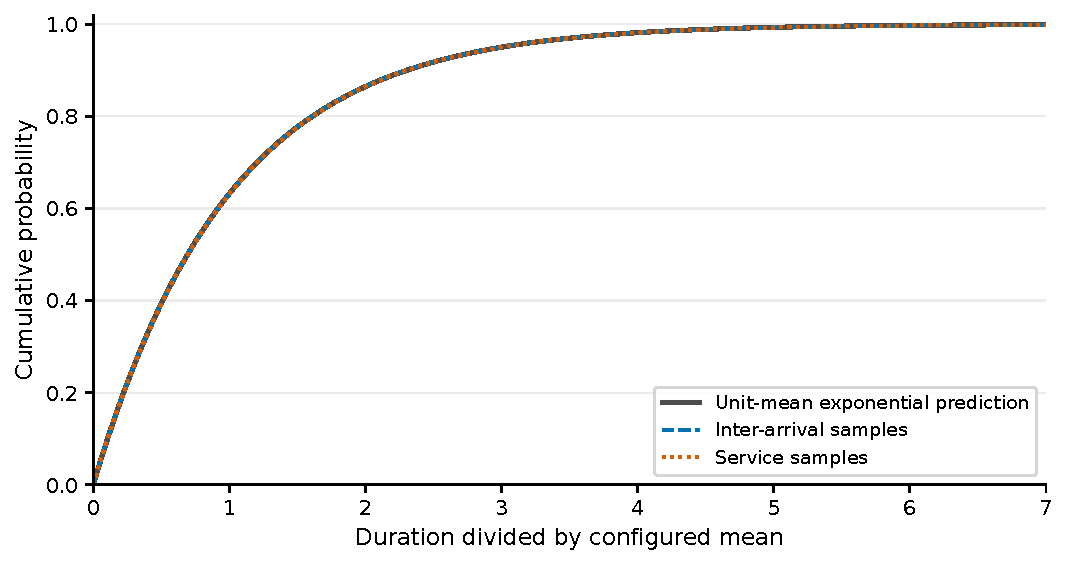
\includegraphics[width=0.98\linewidth]{figures/model_exponential_cdf.pdf}
\caption{E2A distribution check for repeat 1 at the highest configured utilisation. Empirical CDFs use all measurement-cohort inter-arrival intervals and service draws; the theoretical CDF is $1-e^{-x}$.}
\label{fig:model_exponential_cdf}
\end{figure}


Across all runs, the inter-arrival coefficient of variation ranged from 0.990 to 1.009, and the service coefficient of variation ranged from 0.987 to 1.011; an exponential distribution has coefficient of variation 1. The largest absolute same-job arrival/service correlation was 0.0114. The saved diagnostics also include lagged correlations, quantiles and Kolmogorov--Smirnov distances. Of the 40 configured-distribution tests, 0 had an unadjusted asymptotic $p<0.05$. These multiple diagnostic tests are reported without discarding or rerunning data; individual rejections can occur under the specified model.

\subsubsection{Mean delay and population against theory}

Figure~\ref{fig:model_mean_delay} compares each run's mean admission-to-completion time with the configured-rate M/M/1 prediction. Figure~\ref{fig:model_occupancy} independently compares the event-integrated mean system population with its prediction.

\begin{figure}[H]\centering
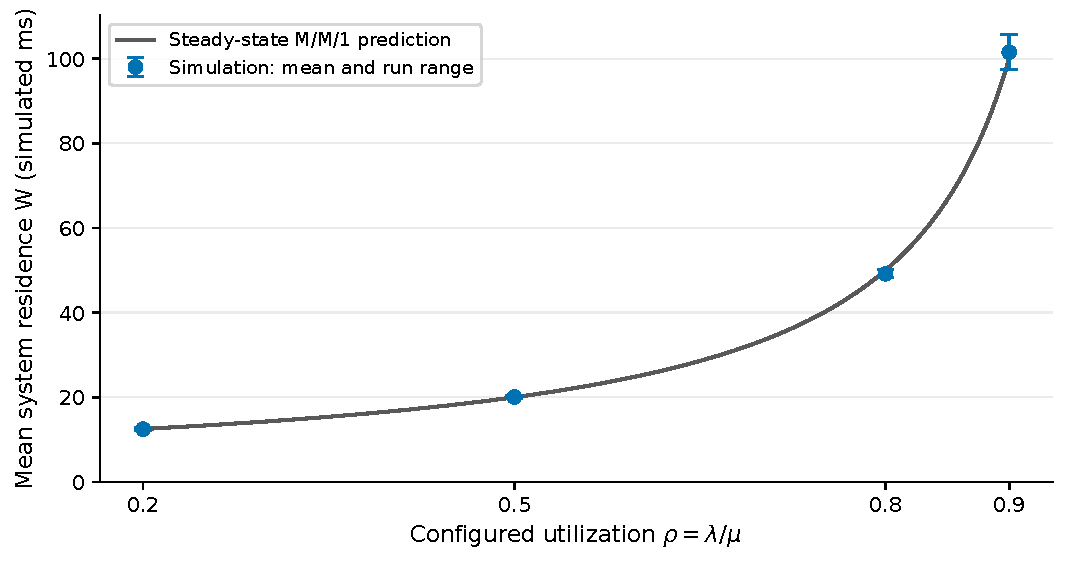
\includegraphics[width=0.98\linewidth]{figures/model_mean_delay.pdf}
\caption{E2A mean system residence against configured-rate M/M/1 theory. Points are means of five runs; bars show the run range. Durations are simulated milliseconds.}
\label{fig:model_mean_delay}
\end{figure}


The absolute relative difference between the mean simulated residence and theory ranged from 0.15\% to 1.67\% across the four settings. Delay grows as utilisation approaches one because successive arrivals increasingly find unfinished work. The finite observation periods and independent realisations produce variation around the steady-state prediction; the comparison is calibration of the controlled model, not a prediction for the real mixed-payload REST service.

\begin{figure}[H]\centering
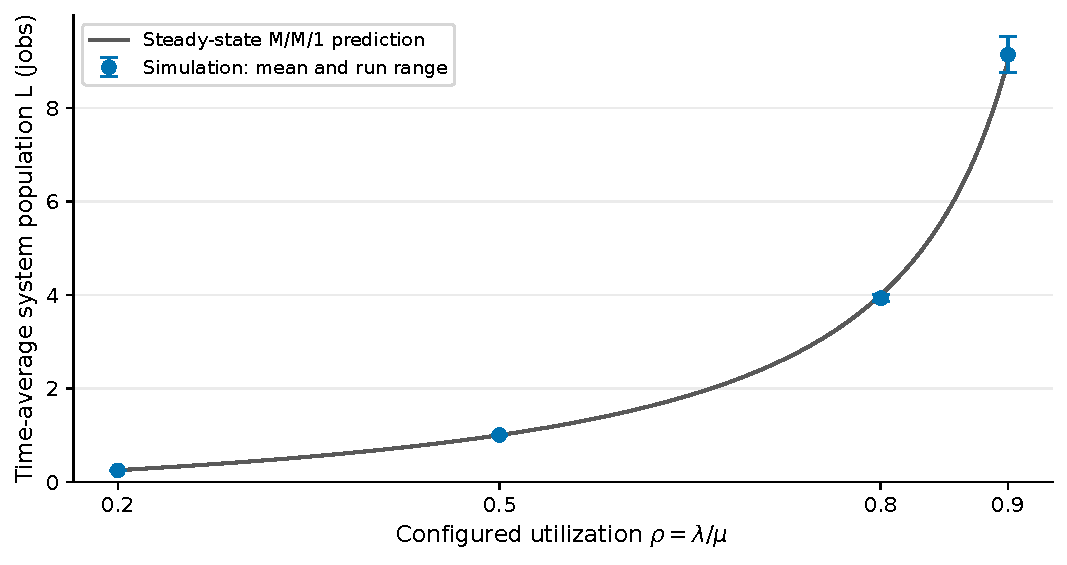
\includegraphics[width=0.98\linewidth]{figures/model_occupancy.pdf}
\caption{E2A system population from exact population-event integration, compared with $L=\rho/(1-\rho)$. The queue includes waiting jobs; the system additionally includes the job in service.}
\label{fig:model_occupancy}
\end{figure}


\begin{table}[H]\centering
\small
\setlength{\tabcolsep}{5pt}
\begin{tabular}{lrrrrr}
\hline
$\rho$ & $W$ (ms) & Theory $W$ (ms) & $L$ & $L_q$ & Busy \\
\hline
0.2 & 12.481 & 12.500 & 0.248 & 0.050 & 0.198 \\
0.5 & 20.064 & 20.000 & 1.004 & 0.503 & 0.501 \\
0.8 & 49.163 & 50.000 & 3.931 & 3.133 & 0.798 \\
0.9 & 101.519 & 100.000 & 9.137 & 8.237 & 0.900 \\
\hline
\end{tabular}
\caption{E2A mean run statistics. Busy is a fraction of measurement time, not process CPU utilisation.}
\label{tab:model_means}
\end{table}

\subsection{Finite-window accounting and Little's relationship}

Little's steady-state relationship is $L=\lambda W$ for consistent populations and time boundaries \cite{little1961}. A finite observation window also intersects jobs admitted before it or completed after it. Let $A_{\rm in}$ be the in-window residence area from jobs admitted before the window, and $A_{\rm out}$ the post-window residence area of jobs admitted inside it. With $T$ the window duration and $\lambda_a$ the admission-cohort count divided by $T$, the exact identity is

\[ L=\lambda_a\overline{W}+(A_{\rm in}-A_{\rm out})/T. \]

The same interval decomposition applies to $L_q$ and $\overline{W_q}$. It is a sample-path accounting check, not an assumption that a finite run is in equilibrium. Exact conservation also requires initial population plus admissions to equal departures plus final population. The raw validators check both identities independently.

\begin{table}[H]\centering
\small
\setlength{\tabcolsep}{5pt}
\begin{tabular}{lrrrr}
\hline
Study / condition & $L$ & $\lambda_a\overline{W}$ & Boundary term & Max. residual \\
\hline
E2A, 0.2 & 0.24838 & 0.24836 & 0.00002 & 0.0e+00 \\
E2A, 0.5 & 1.00424 & 1.00421 & 0.00004 & 1.9e-16 \\
E2A, 0.8 & 3.93130 & 3.93132 & -0.00002 & 1.1e-15 \\
E2A, 0.9 & 9.13696 & 9.13646 & 0.00049 & 2.4e-15 \\
E2B, Staggered & 0.68170 & 0.68170 & 0.00000 & 0.0e+00 \\
E2B, Synchronized & 3.44074 & 3.44074 & 0.00000 & 0.0e+00 \\
E2B, Poisson & 1.26915 & 1.26914 & 0.00002 & 0.0e+00 \\
E2B, Bursty ON/OFF & 29.10004 & 29.10004 & 0.00000 & 0.0e+00 \\
\hline
\end{tabular}
\caption{Finite-window system accounting. First three numerical columns are means of five runs; the last is the largest absolute identity residual in that condition, expressed in jobs/messages. Rounding displayed columns can obscure small corrections.}
\label{tab:little}
\end{table}

The maximum E2A system-identity residual was 2.39e-15 jobs, at floating-point precision. In E2B, the maximum difference between the independently integrated system events and the summed clipped per-message residence intervals was 0 message-nanoseconds. E2B shares an integer-nanosecond timestamp between each state change and its message record, so this check can be exact. Agreement validates the measurement boundary and accounting; it does not establish that E2B has exponential service times.

\subsection{E2B procedure: vary arrival timing at fixed expected workload}

Four actual ROS 2 source nodes run in one open-loop publisher process. Each node publishes command, status, odometry and sensor streams at expected rates 2, 5, 20 and 5 messages/s, with synthetic x-filled payload strings of 100, 100, 250 and 20,000 bytes. ROS topics carry \texttt{std\_msgs/String} messages containing the JSON envelope and payload string; the four class names denote traffic profiles, not native ROS message definitions. Thus the expected aggregate arrival rate is 128 messages/s. The payload mixture is fixed in expectation; Poisson realisations have small count and composition variation, which is retained in the per-source and per-class tables. JSON metadata increases HTTP body bytes beyond these payload-string sizes.

All patterns use the same 1,000-message waiting FIFO, one persistent HTTP/1.1 connection, one server worker, no retries and an unshaped isolated virtual-Ethernet path in WSL. A fixed 4.0 ms hold is requested inside each server operation. The realised gateway service $S$ also includes serialization, HTTP transport, response handling and scheduling, so it is neither exactly that hold duration nor assumed exponential. Source scheduling does not wait for HTTP responses.

\begin{table}[H]\centering
\small
\setlength{\tabcolsep}{5pt}
\begin{tabular}{p{0.23\linewidth}p{0.69\linewidth}}
\hline
Arrival pattern & Definition \\
\hline
Staggered periodic & Deterministic per-stream periods; phases staggered over the 16 streams. \\
Synchronized periodic & The same periods, with every stream assigned zero phase. \\
Poisson & Independent exponential inter-arrival durations per source and class. \\
Bursty ON/OFF & A shared 1 s cycle: Poisson arrivals at $5\times$ rate for 0.2 s, then no arrivals for 0.8 s. \\
\hline
\end{tabular}
\caption{E2B arrival definitions. The bursty schedule has deterministic ON/OFF durations and is not a Markov-modulated Poisson process.}
\label{tab:patterns}
\end{table}

Each pattern has five repetitions, with seeded shuffled run order, 20 s warmup, 120 s measurement and up to 60 s drain. Warmup and measurement contain whole ON/OFF cycles, giving the bursty and ordinary Poisson cases identical integrated expected arrivals over each window. The realised number of Poisson arrivals remains random. The ROS graph, source scheduler timestamps, gateway events, server records, CPU samples and packet captures are retained per run. A separate validator reconstructs schedules, checks actual node/topic counts, verifies FIFO/concurrency and reconciles message identities, timing, populations and outcomes.

Strict capture checks passed for all 20 live runs and matched 358,031 complete HTTP exchanges, including warmup and drain. Capture drops totalled 0. This cross-check validates captured request/response identities and byte accounting; it does not turn packet capture into a claim about physical-network performance.

Simultaneous scheduled events are ordered by scheduled time, source ID, class name and sequence number; the class tie order is command, odometry, sensor, then status. The source publishes in this deterministic schedule order. ROS callback order is observed separately and is not assumed to reproduce every tie. This convention matters for class-level delays in synchronized batches. The 100 ms arrival bins resolve the ON/OFF cycle; one-second bins alone would integrate a complete burst cycle and conceal its concentration.

\subsubsection{First verify the offered workload}

Figure~\ref{fig:live_rates} uses published-message counts, gateway admissions and completed responses within each measurement window, each divided by the window duration. Differences at a boundary need not imply loss; message-level accounting follows the admission cohort through drain.

\begin{figure}[H]\centering
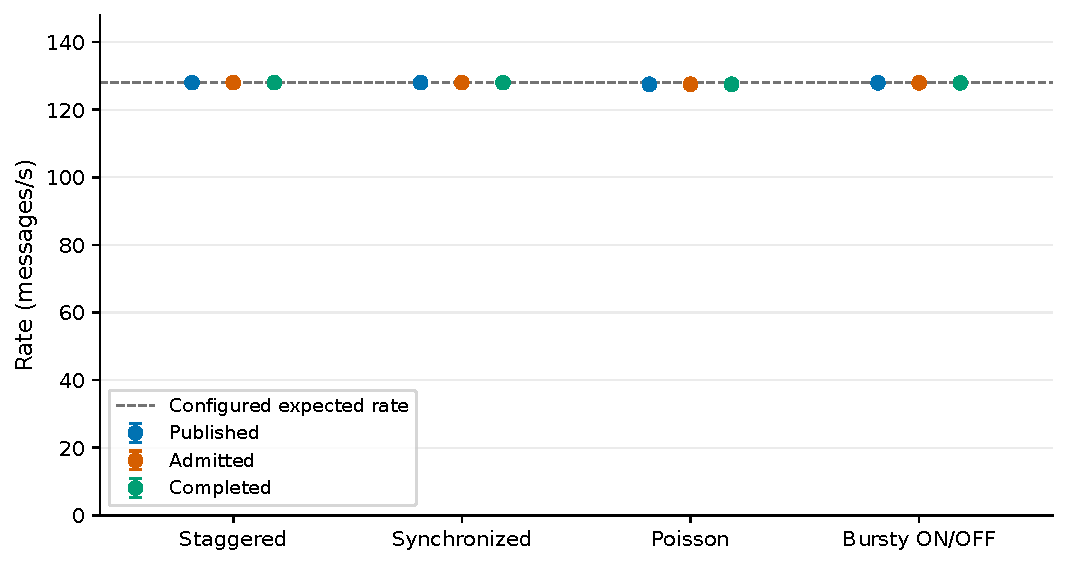
\includegraphics[width=0.98\linewidth]{figures/live_rates.pdf}
\caption{Realised E2B workload and completion rates. The dashed line is the configured expected aggregate rate of 128 messages/s. Bars are the range of five run rates.}
\label{fig:live_rates}
\end{figure}


The condition-mean admission rates ranged from 127.55 to 128.00 messages/s. Across all 20 runs, 306,896 source-cohort messages were generated, with 0 FIFO drops and 0 combined request errors, missing ROS messages or unresolved source-cohort messages after drain. Expected average load is held fixed; the plot and saved class counts show the realised load rather than forcing stochastic counts to match.

\subsubsection{Arrival patterns become different queue histories}

Figure~\ref{fig:live_arrival_trace} bins source-publication timestamps into 100 ms intervals. Figure~\ref{fig:live_queue_trace} uses the exact admission/dequeue/completion event log to draw the waiting-queue state. Both use the first 10 measurement seconds of repeat 1 for every pattern. They illustrate timing mechanisms; full-window statistics below support the comparison.

\begin{figure}[H]\centering
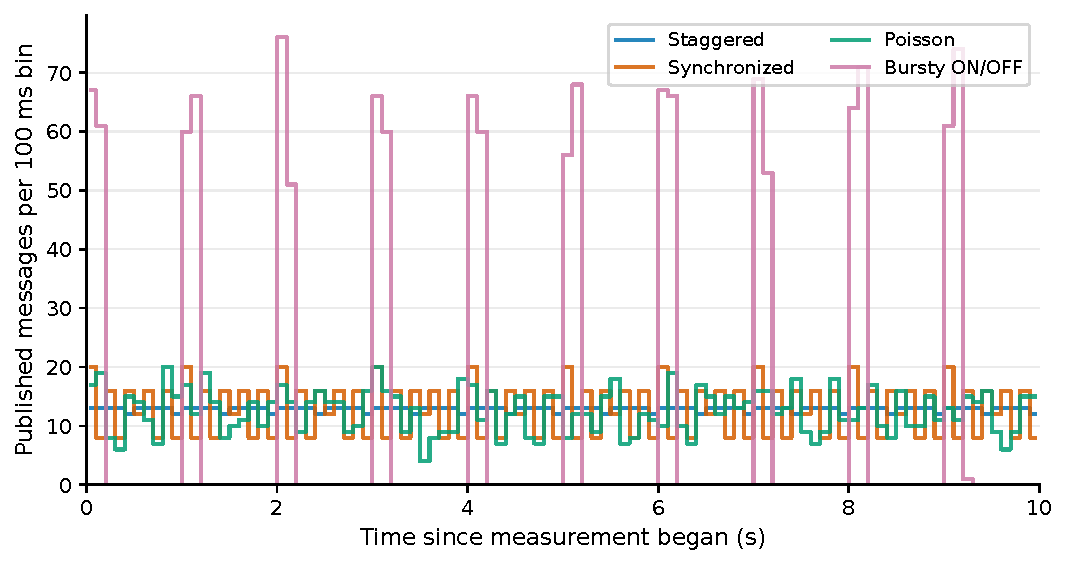
\includegraphics[width=0.98\linewidth]{figures/live_arrival_trace.pdf}
\caption{Example source-publication counts in non-overlapping 100 ms bins. Each line is repeat 1 of one arrival pattern; individual source classes are mixed in the aggregate count.}
\label{fig:live_arrival_trace}
\end{figure}


\begin{figure}[H]\centering
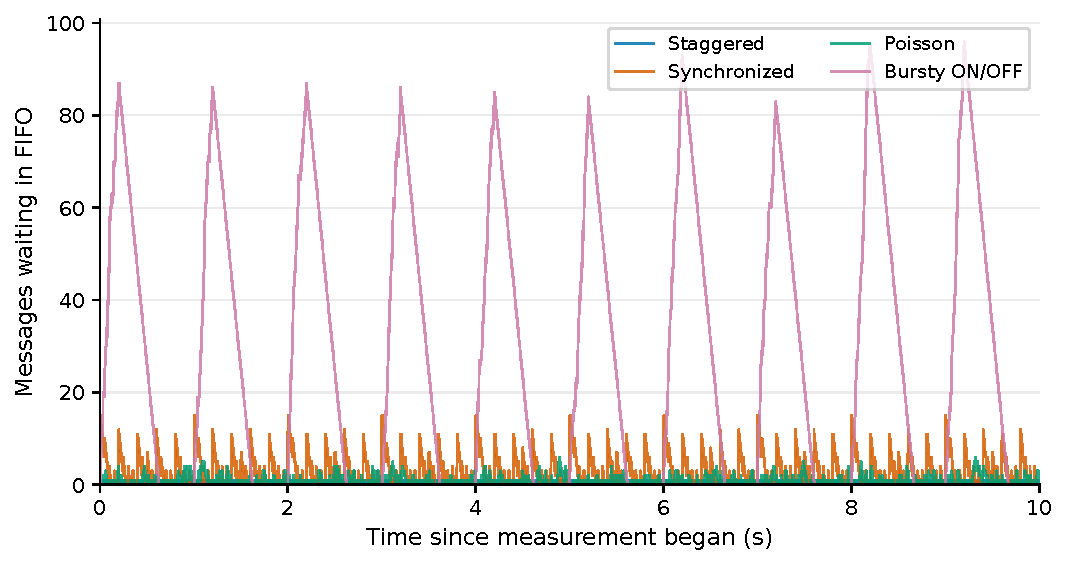
\includegraphics[width=0.98\linewidth]{figures/live_queue_trace.pdf}
\caption{Example waiting-queue histories for the same fixed repeat and interval. A step changes only at a logged gateway event; a job in service is excluded from the waiting population.}
\label{fig:live_queue_trace}
\end{figure}


A server processes one message at a time, so arrivals accumulated during a busy interval must wait. Synchronized periodic sources can produce short simultaneous batches; the ON/OFF case concentrates each second's expected demand into its first fifth. Idle portions of the cycle do not erase the waiting time experienced by messages in the preceding burst. The realised traces, rather than the configured labels alone, establish how these effects appeared in this implementation.

\subsubsection{Waiting time, tails and occupancy}

Figures~\ref{fig:live_wait} and~\ref{fig:live_system_delay} use the gateway-admission cohort and include completions during drain. Their p95 and p99 values describe successful admitted messages; loss is reported alongside them so a favourable tail cannot be obtained by hiding discarded messages.

\begin{figure}[H]\centering
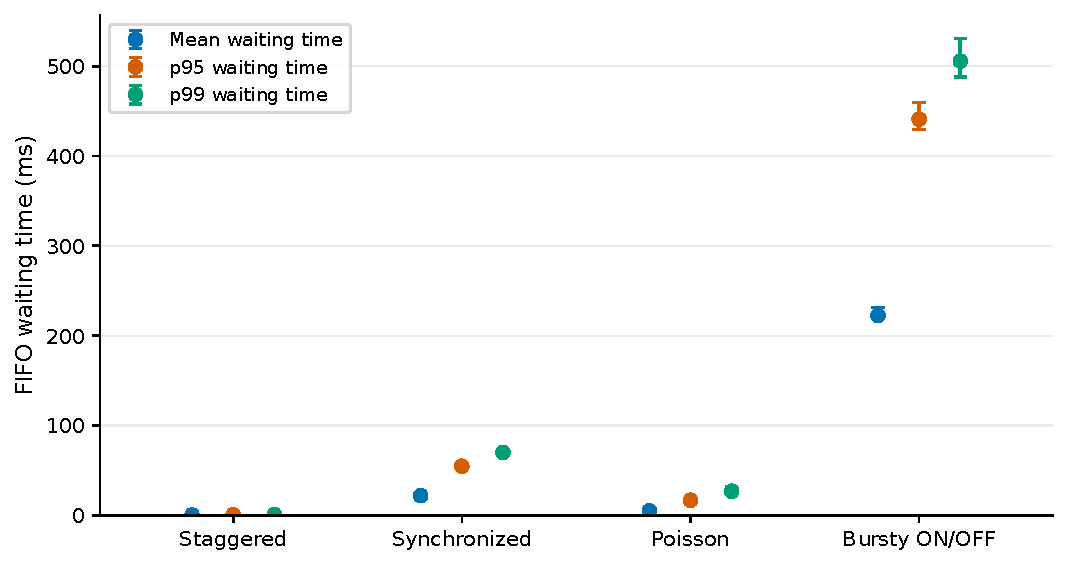
\includegraphics[width=0.98\linewidth]{figures/live_wait.pdf}
\caption{E2B mean, p95 and p99 FIFO waiting time. Waiting runs from admission to worker dequeue. Each point averages the corresponding statistic over five runs; bars show their range.}
\label{fig:live_wait}
\end{figure}


\begin{figure}[H]\centering
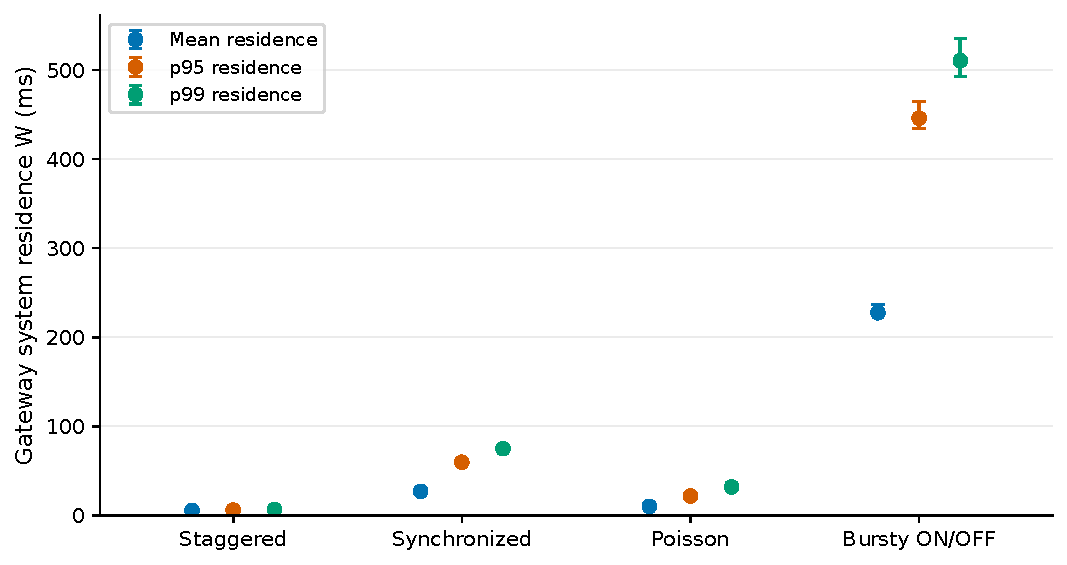
\includegraphics[width=0.98\linewidth]{figures/live_system_delay.pdf}
\caption{E2B residence from gateway admission to response-handling completion. This adds service to waiting; it excludes the source-to-gateway delivery interval.}
\label{fig:live_system_delay}
\end{figure}


The lowest condition-mean gateway p95 was 5.79 ms for staggered, and the highest was 446.03 ms for bursty on/off. These are observed differences under the fixed shared gateway, not a universal ranking of arrival processes. The realised mean service times ranged from 4.956 to 5.011 ms across conditions despite the same requested server hold; differences in scheduling or overhead can contribute alongside arrival variability.

\begin{figure}[H]\centering
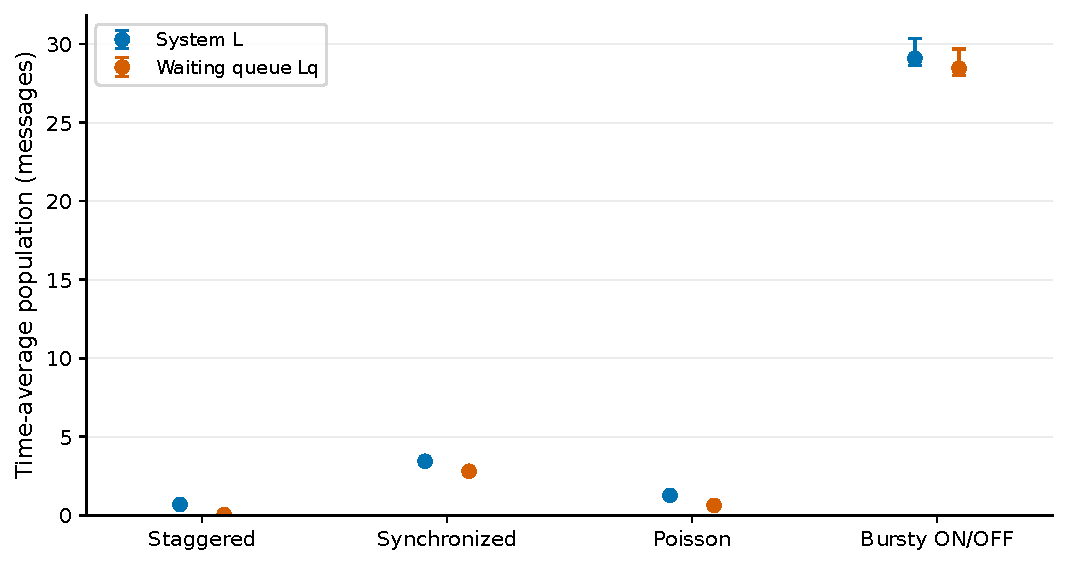
\includegraphics[width=0.98\linewidth]{figures/live_occupancy.pdf}
\caption{E2B time-average system and waiting-queue populations from exact event integration. The difference between the two populations equals the single-worker busy fraction.}
\label{fig:live_occupancy}
\end{figure}


\begin{table}[H]\centering
\small
\setlength{\tabcolsep}{5pt}
\begin{tabular}{lrrrrr}
\hline
Pattern & $W$ (ms) & $W_q$ (ms) & $S$ (ms) & $L_q$ & Busy (\%) \\
\hline
Staggered & 5.33 & 0.31 & 5.011 & 0.040 & 64.14 \\
Synchronized & 26.88 & 21.90 & 4.985 & 2.803 & 63.80 \\
Poisson & 9.95 & 4.95 & 5.004 & 0.631 & 63.82 \\
Bursty ON/OFF & 227.43 & 222.47 & 4.956 & 28.466 & 63.42 \\
\hline
\end{tabular}
\caption{E2B means of five run-level values. The latency decomposition uses one common admission cohort; occupancy and busy fraction use the measurement-time window.}
\label{tab:live_means}
\end{table}

\subsubsection{Check service, scheduling and class-level consequences}

\begin{table}[H]\centering
\small
\setlength{\tabcolsep}{5pt}
\begin{tabular}{lrrrr}
\hline
Pattern & CV$(S)$ & IAT CV & Lag p95 (ms) & CPU (\%) \\
\hline
Staggered & 0.050 & 0.363 & 0.174 & 4.5 / 17.4 / 6.2 \\
Synchronized & 0.055 & 2.283 & 1.958 & 2.6 / 10.3 / 5.8 \\
Poisson & 0.055 & 1.014 & 0.191 & 4.1 / 15.4 / 6.0 \\
Bursty ON/OFF & 0.060 & 9.072 & 0.221 & 2.7 / 11.8 / 5.5 \\
\hline
\end{tabular}
\caption{Variability and execution checks, averaged over runs. IAT CV is the gateway inter-arrival coefficient of variation. The three CPU values are source / gateway / server: process CPU time divided by wall time, expressed relative to one logical core. Source lag is scheduled-to-source timestamp delay.}
\label{tab:live_checks}
\end{table}

The service coefficient of variation and source scheduling lag test how well the implementation follows the intended model. An exponential service distribution would have coefficient of variation near one; a deterministic hold plus real processing overhead does not create M/M/1 merely because one arrival schedule is Poisson. Accordingly, no M/M/1 fitted curve is overlaid on E2B. The service boundary includes the occupied sender while it waits for the HTTP response, so busy fraction is distinct from CPU utilisation.

\begin{table}[H]\centering
\small
\setlength{\tabcolsep}{5pt}
\begin{tabular}{lrrrr}
\hline
Pattern & Command & Status & Odometry & Sensor \\
\hline
Staggered & 0.00 & 0.00 & 0.00 & 0.00 \\
Synchronized & 0.00 & 0.00 & 0.00 & 0.00 \\
Poisson & 0.00 & 0.00 & 0.00 & 0.00 \\
Bursty ON/OFF & 78.89 & 55.63 & 78.37 & 0.00 \\
\hline
\end{tabular}
\caption{Mean run deadline-miss percentage, by class. Denominators include all generated messages of that class in the source-time window; late success, loss and non-completion count as misses. Targets are 100, 200, 100 and 1,000 ms for command, status, odometry and sensor, respectively. These are illustrative project targets, not certified application requirements.}
\label{tab:class_deadlines}
\end{table}

For bursty ON/OFF arrivals, the mean deadline-miss percentages were 78.89\% for command, 55.63\% for status, 78.37\% for odometry and 0.00\% for sensor. Together with the loss and completion counts, these class-level results distinguish eventual delivery from timely delivery. An average offered rate below the worker's capacity can still produce long waits within a concentrated burst, and classes with different deadline thresholds can therefore experience different practical consequences.

\subsection{Interpretation, limits and reproducibility}

E2A checks the queue model and the analysis pipeline under explicit exponential assumptions. E2B then isolates arrival timing at a fixed expected mixed-payload workload and fixed service setup. The event-level Little identity provides a common accounting check without asserting that the empirical service is exponential or that every finite window is in steady state. The evidence supports conclusions about this measured shared FIFO implementation and these four specified arrival schedules.

The sources, gateway and server share one WSL host; the virtual link has no physical propagation path or competing external traffic. Four actual ROS nodes are not four independent computers, and one publishing process shares a scheduler. The fixed server hold is an intentional controlled service cost. Five repetitions show run variation but do not establish a confidence interval, and 120 s windows do not characterise every rare tail event. Independent HTTP-client scaling, topology selection under E9, different network impairments and other protocol variants remain separate experiments.

The deliverable includes one plot per PDF, per-run and aggregate CSV tables, this reusable LaTeX section and the standalone report. The raw datasets retain the frozen settings, code snapshots/hashes, seeds, jobs or message records, event logs, validation and captures. \texttt{report\_evidence.json} records SHA-256 hashes of the report's consumed inputs and generator. Rebuild figures from the validated datasets with \texttt{scripts/report\_e2.py}; compile \texttt{main.tex} twice with pdfLaTeX. The individual-run CSVs retain full precision for further analysis.

\subsection{Recommended figures for the main report}

For a concise narrative, retain the model mean-delay plot, the finite-window Little table, the realised-rate plot, the arrival and queue examples, the waiting-time plot and the occupancy plot. Together they establish the model, verify comparable input workload, show the timing mechanism, quantify its effect and check the accounting. Put the exponential CDF, system-tail plot, detailed service checks and class-level table in supplementary material if space is limited.
